\chapter{Математическое описание системы и постановка задачи}
\label{cha:design}

Для синтеза алгоритма управления кооперативной системы из двух артикулированных шестизвенных манипуляторов формализуем ее кинематической и динамической модели. Кинематика каждого манипулятора описывается в соответствии с соглашением Денавита – Хартенберга \cite{Spong2006}.
Обозначения для кинематических параметров артикулированного робота-манипулятора представлены на рисунке \ref{fig:dh_convention}.

\begin{figure}[ht!]
  \centering
  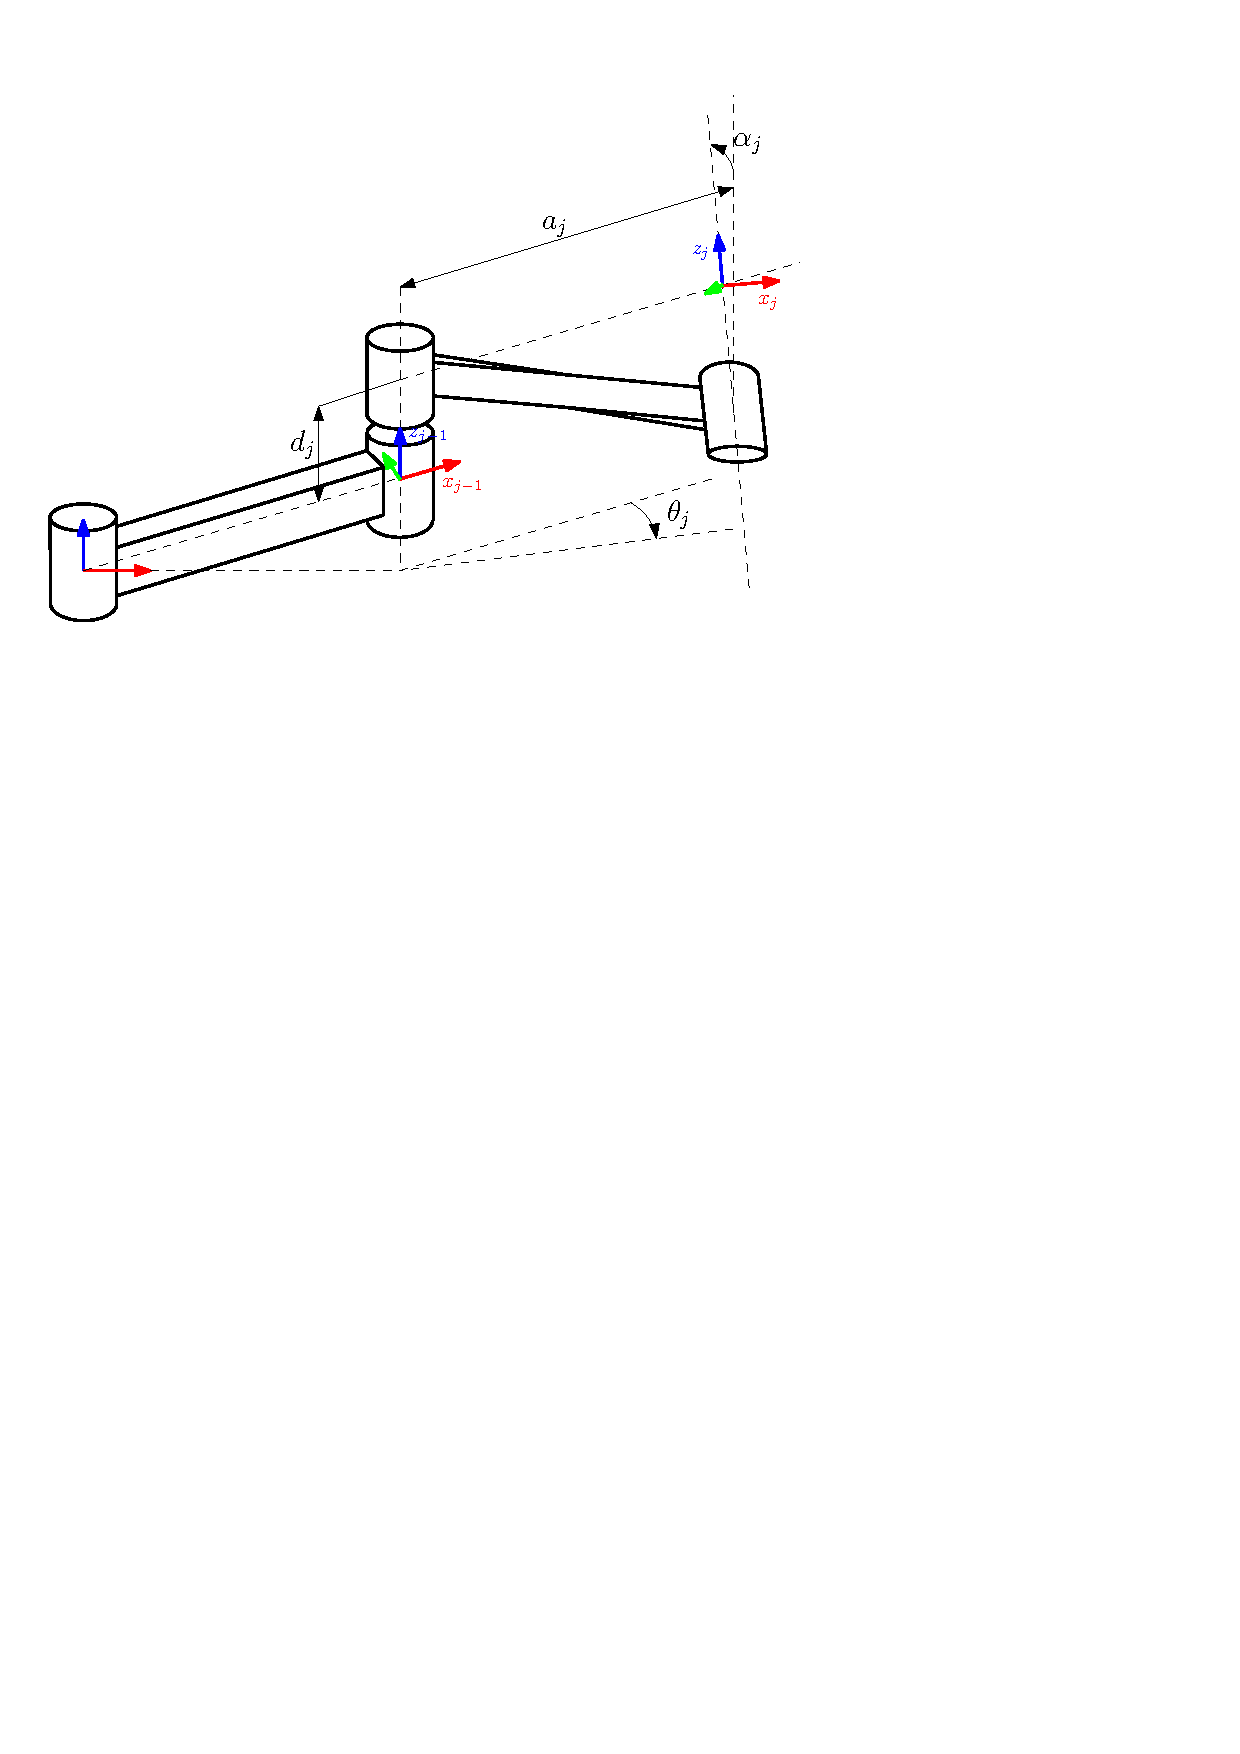
\includegraphics[width=0.7\textwidth]{inc/img/dh_convention}
  \caption{Описание параметров Денавита-Хартенберга}
  \label{fig:dh_convention}
\end{figure}

Для синтеза алгоритма кооперативного управления ограничимся рассмотрением кооперации двух артикулированных манипуляторов, т.е $k=2$. Осуществленный в последующем разделе синтез справедлив и для систем с большим числом агентов $k$. Стоит отметить, что полученный алгоритм требует модификации для управления избыточными манипуляторами.

\section{Кинематика кооперативной системы}
\label{coop_kin}
Координаты рабочего инструмента каждого манипулятора могут быть получены из решения прямой задачи кинематики:
\begin{equation}
  p_i(q_i) = \begin{bmatrix}  o_{6,i}(q_i) \\ \varphi_i(q_i) \end{bmatrix},\quad i = \overline{1,2}\ ,
\end{equation}
где $p_i \in \R_{6\times1}$ --- вектор состоящий из вектора координат $o_{6,i} \in \R_{3\times1}$ и ориентаций(углов Эйлера) $\varphi_i \in \R_{3\times1}$ рабочего инструмента $i$-го манипулятора в базовой системе координат, $q_i=\theta_i \in \R_{6\times 1}$ --- вектор угловых положений сочленений $i$-го манипулятора.\\

Для определения скорости движения объекта манипулирования введем понятие относительной матрицы Якоби $i$ - го манипулятора:
\begin{equation*}
      J_{r,i} = \begin{bmatrix} z_{0,i}\times(x_o - o_{0,i}) & \dots & z_{5,i}\times(x_o - o_{5,i})\\
      z_{0,i} & \dots & z_{5,i} \end{bmatrix},\quad i =\overline{1,2}
\end{equation*}
где $o_{j,i}$ --- вектор координат положения $j$-го сочленения $i$-го манипулятора в базовой системе координат,  $z_{j,i}$ --- орт-вектор оси вращения $j$-го сочленения $i$-го манипулятора, $\displaystyle x_o  = \begin{bmatrix}
  o_o \\ \varphi_o
\end{bmatrix} \in \R_{6\times 1}$ --- координаты и ориентация(углы Эйлера) объекта манипулирования.

В случае жесткого удерживания, т.е когда вектор от начала системы координат объекта, до точки рабочего инструмента постоянен: $r_i=const$, получим следующие кинематические ограничения:
\begin{equation}
   \begin{bmatrix} \upsilon_o \\ \omega_o \end{bmatrix} = J_{r,1}\cdot \dot{q}_1 = J_{r,2}\cdot \dot{q}_2
\end{equation}

Так как измерение положения объекта манипулирования не представляется нам возможным,то примем наиболее часто используемое допущение \cite{Handbook}, что:
\begin{equation}
  x_o = \frac{1}{2}(p_1 + p_2),\quad \begin{bmatrix} \upsilon_o \\ \omega_o \end{bmatrix} = \begin{bmatrix} \frac{1}{2}J_1 & \frac{1}{2}J_2\end{bmatrix}\cdot \dot{q}_c = J_o \cdot \dot{q}_c, \quad q_c = \begin{bmatrix} q_1 \\ q_2\end{bmatrix}
\end{equation}
Стоит отметить также взаимосвязь между вектором $\dot{x}_o$ содержащем производной вектора углов Эйлера и вектором $\begin{bmatrix} \upsilon_o \\ \omega_o \end{bmatrix}$, содержащим значение скоростей вращения вокруг осей $x$, $y$, и $z$ в базовой системе координат:
\begin{equation}
  \quad \dot{x_o} = T_a^{-1} \begin{bmatrix} \upsilon_o \\ \omega_o \end{bmatrix}
\end{equation}
\section{Динамика кооперативной системы}
\label{coop_dyn}
Динамика каждого манипулятора, описывается уравнением \eqref{eq:base_one_manipulator_model} с соответствующим индексом для $i$-го манипулятора:
\begin{equation}
  M_i(q_i)\ddot{q}_i + C_i(q_i,\dot{q}_i)\dot{q}_i + g_i(q_i) = \tau_{c,i} - J_i^\top(q_i) f_{c,i}, \quad i =\overline{1,2} \ ,
  \label{eq:base_i_manipulator_model}
\end{equation}

Для упрощения изложения введем агрегирование векторов и матриц моментов и сил на рабочих инструментах:
\begin{equation}
   J_c = \begin{bmatrix} J_1(q_1) & 0_6\\ 0_6 & J_2(q_2) \end{bmatrix},\quad  \tau_c = \begin{bmatrix} \tau_{c,1}\\ \tau_{c,2} \end{bmatrix} = J_c^\top \cdot F_c
\end{equation}

Распишем более подробно динамическую модель объекта манипулирования, которая в общем виде задана уравнением \ref{eq:obj_base_model}.
Кинетическая энергия объекта манипулирования по теореме Кёнига состоит из кинетической энергии его поступательного и вращательного движения:
\begin{equation}
  K = \frac{1}{2}m_o\cdot \upsilon^\top_o \upsilon_o + \frac{1}{2} \omega_o^\top R I_o R^\top \omega_o
\end{equation}


\section{Постановка задачи}
Для заданной в предыдущих пунктах \ref{coop_kin} и \ref{coop_dyn} кооперативной системы из двух артикулированных роботов-манипуляторов синтезировать алгоритм гибридного позиционного/силомоментного управления для удержания объекта в заданном положении с желаемым контактным усилием при условии отсутствии знаний динамических параметров объекта манипулирования.

%
%
% \paragraph{Проверка} параграфа. Вроде работает.
% \paragraph{Вторая проверка} параграфа. Опять работает.
%
% Вот.
%
% \begin{itemize}
% \item Это список с <<палочками>>.
% \item Хотя он и по ГОСТ, но\dots
% \end{itemize}
%
% \begin{enumerate}
% \item  Для списка, начинающегося с заглавной буквы, лучше список с цифрами.
% \end{enumerate}
%
% Формула \eqref{F:F1} совершено бессмысленна.
%
% %Кстати, при каких-то условиях <<удавалось>> получить двойный скобки вокруг номеров формул. Вопрос исследуется.
%
% \begin{equation}
% a= cb
% \label{F:F1}
% \end{equation}
%
% А формула~\eqref{eq:fourierrow} имеет некоторый смысл.
% Кроме этого она пытается иллюстрировать применение окружения \Code{eqndesc} которое размещает формулу совместно с её описанием.
% Однако обратите внимание на нумерацию формул~\eqref{eq:fourierrow} и \eqref{F:F2}, попробуйте добавить \Code{[H]} к такой формуле.
%
% \begin{eqndesc}
%     \begin{equation}\label{eq:fourierrow}
%         f(x) = \frac{a_0}{2} + \sum\limits_{k=1}^{+\infty} A_k\cos\left(k\frac{2\pi}{\tau}x+\theta_k\right)
%     \end{equation}
%
%     где $A_k$ "--- амплитуда  k-го гармонического колебания,\\
%     $A_k$ "--- амплитуда $k$-го гармонического колебания,\\
%     $ k\frac{2\pi}{\tau} = k\omega$ "--- круговая частота гармонического колебания,\\
%     $\theta_k$ "--- начальная фаза $k$-го колебания.
% \end{eqndesc}
%
%
% Окружение \texttt{cases} опять работает (см. \eqref{F:F2}), спасибо И. Короткову за исправления..
%
%
% \begin{equation}
% a= \begin{cases}
%  3x + 5y + z, \mbox{если хорошо} \\
%  7x - 2y + 4z, \mbox{если плохо}\\
%  -6x + 3y + 2z, \mbox{если совсем плохо}
% \end{cases}
% \label{F:F2}
% \end{equation}
%
% \section{Подсистема всякой ерунды}
%
% Культурная вставка dot-файлов через утилиту dot2tex (рис.~\ref{fig:fig02}).
%
% \begin{figure}
%   \centering
% % [width=0.5\textwidth] --- регулировка ширины картинки
%   \includegraphics[width=.5\textwidth]{inc/dot/cow2}
%   \caption{Рисунок}
%   \label{fig:fig02}
% \end{figure}
%
%
% \subsection{Блок-схема всякой ерунды}
%
% \subsubsection*{Кстати о заголовках}
%
% У нас есть и \Code{subsubsection}. Только лучше её не нумеровать.

%%% Local Variables:
%%% mode: latex
%%% TeX-master: "rpz"
%%% End:
